\documentclass{article}

\begin{document}


\setlength{\parindent}{6ex}


\begin{figure}
    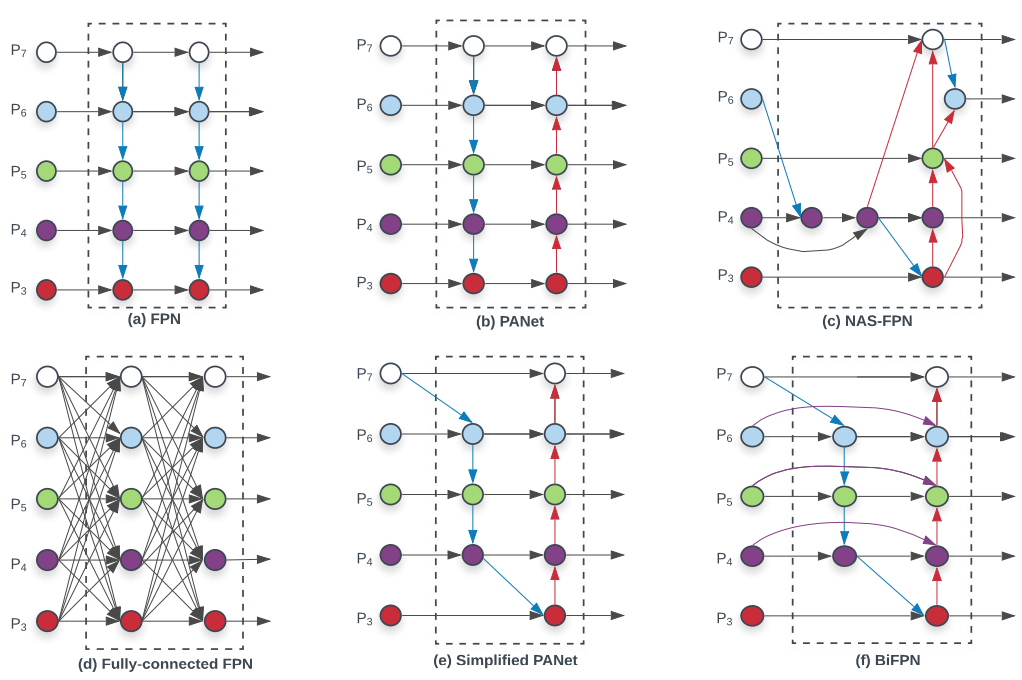
\includegraphics[width=\textwidth]{evoloffpn}
    \caption{Feature Network Design \cite{efficientdetcite}. 
    As it can be seen in this figure, FPN introduces a top-down pathway to fuse multi-scale 
    features from level 3 to level 7 (P3-P7). Then, PANet introduces an additional bottom-up 
    pathway. NAS-FPN introduces a method in which a neural architecture is used to find an 
    irregular network topology. Fully-connected FPN adds expensive connections from all input 
    features to output features. Simplified PANet removes the nodes if they only have one input 
    edge. BiFPN is discussed in this paper and it is introduced with better accuracy and efficieny 
    trade-offs.}
    \label{fig:bifpn1}
\end{figure}

\begin{figure}
    \centering
    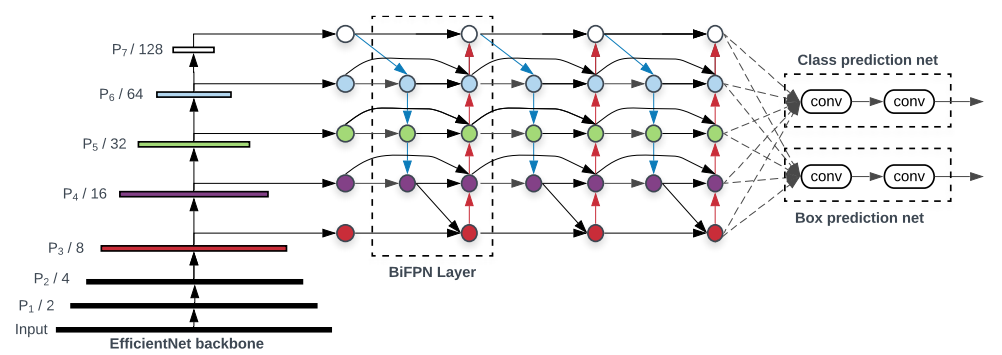
\includegraphics[width=\textwidth]{models/efficientdetnet}
    \caption{Network of EfficientDet \cite{efficientdetcite}. Its backbone network is EfficientNet 
    and BiFPN is used as feature network. After the backbone and feature networks, shared class 
    and box prediction networks are used to predict. Both BiFPN and class/box prediction layers 
    are used multiple times based on the constraints as shown in figure \ref{fig:efficientdetscale1}.}
    \label{fig:efficientdetnet1}
\end{figure}

\indent

This article aims to study model efficiency and increase model 
efficiency. Therefore, building a scalable architecture with both higher 
accuracy and efficiency \cite{efficientdetcite} is studied. As you can see in figure 
\ref{fig:bifpn1}, variations of FPN are studied and BiFPN is chosen as the best-performing 
one. Also, as you can see in figure \ref{fig:efficientdetnet1}, EfficientDet is developed 
using EfficientNet as a backbone, BiFPN as a feature extractor, and two subnetworks 
one responsible for class prediction, the other one responsible for bounding 
box prediction. \par

There are two main ideas in the design of BiFPN: efficient bidirectional 
cross-scale connections and weighted feature fusion. Difference between 
FPN and BiFPN can be observed in figure \ref{fig:bifpn1}. FPN has one-way 
data flow but bidirectional data flow is observed to be better. Also, 
the nodes that have only one input node are removed since there is no 
feature fusion and that node will have less contribution to feature network. 
In addition, an extra edge is added from input nodes to output nodes. The 
reason is to fuse more features. Finally, to enable more high-level feature, 
same layer is applied multiple times as you can see in \ref{fig:efficientdetnet1}.
The importance of multi-scale feature fusion is mentioned before. The novel contribution 
here is using weights for feature fusion. Previous fusing operations 
on feature maps does not include weights until BiFPN, therefore, all the 
input features contribute equally. The problem here is that different 
input feature on different resolutions does not contribute output feature 
equally. Therefore, a weighted feature fusion is needed to obtain a better 
performance. Thus, learnable parameters are present to learn the importance 
of different features. \par

Bigger backbone networks or higher input resolutions can lead to an increase 
in accuracy but also, can lead to a decrease in efficiency due to the high 
number of operations required. Therefore, scaling up the network is crucial 
to obtain both accuracy and efficiency. The scaling component $\phi$ is used. 
You can see the configurations in figure \ref{fig:efficientdetscale1}. 
When detector configured from D0 to D7, mean average precision increases but 
also the inference time for the detector to run increases. The required model 
can be chosen based on the task performed. 

\begin{figure}
    \centering
    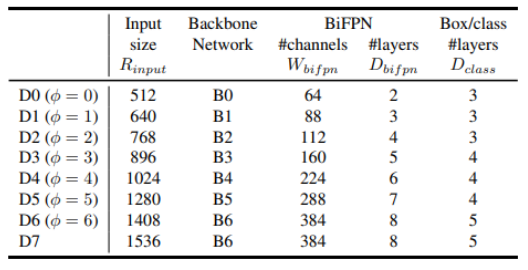
\includegraphics[width=\textwidth]{efficientdetscale}
    \caption{Scaling Table of EfficientDet D0-D7 \cite{efficientdetcite}. $\phi$ is used as 
    the compound coefficient that controls all other scaling dimensions.}
    \label{fig:efficientdetscale1}
\end{figure}

\end{document}